\documentclass{standalone}
\usepackage{tikz}
\usepackage{ctex,siunitx}
\setCJKmainfont{Noto Serif CJK SC}
\usepackage{tkz-euclide}
\usepackage{amsmath}
\usetikzlibrary{patterns, calc,3d}
\usetikzlibrary {decorations.pathmorphing,decorations.pathreplacing,decorations.shapes}
\tikzset{label style/.append style={font=\small}}
\begin{document}
\small
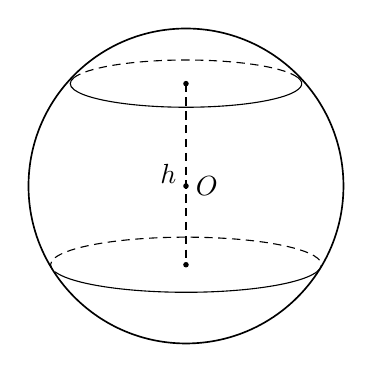
\begin{tikzpicture}[>=latex,scale=1.0]
  \draw[semithick](0,0)circle(2);
  \fill[black](0,0)circle(1pt)node[right]{$O$};
  \fill[black](0,1.3)circle(1pt)(0,-1.0)circle(1pt);
  \draw[draw=none](0,1.3)--++({1.47*cos(15)},{0.3*sin(15)}) coordinate (A);
  \draw[draw=none](0,-1)--++({1.72*cos(-15)},{0.35*sin(-15)}) coordinate (B);
  \draw[densely dashed](0,1.3)--(0,-1)node[midway,left]{$h$};
  \draw(A)arc(15:-195:1.47 and 0.3);
  \draw(B)arc(-15:-165:1.72 and 0.35);
  \draw[densely dashed](A)arc(15:165:1.47 and 0.3);
  \draw[densely dashed](B)arc(-15:195:1.72 and 0.35);
\end{tikzpicture}
\end{document}